\chapter{Analisi dei requisiti}
Si vuole realizzare un database atto al supporto e alla gestione del personale di controllo del traffico aereo.
\section{Intervista}
Un primo testo ottenuto dall'intervista è il seguente (Estrema semplificazione rispetto ad un caso reale):\\
Si richiede di creare uno strumento che permetta di allocare i turni di lavoro delle rispettive posizioni. La giornata è suddivisa in 3 turni da 8 ore (8:00, 16:00, 24:00), dopo ogni turno lavorativo un controllore deve avere almeno 3 turni di riposo prima di tornare al lavoro, per un massimo di 300 turni annuali.
Esistono 3 tipi di posizioni, ognuna relativa ad un segmento della tratta di volo diverso. 
\begin{itemize}
    \item Aerodromo:
I punti di partenza e di arrivo delle tratte, ogni aerodromo ha una o più piste e una o più posizioni di tipo (Delivery, si occupa di fornire clearance IFR; Ground, si occupa di gestire traffico al suolo; Tower, si occupa di gestire gli aeromobili sulle piste.)
\item Avvicinamento:
Sono posizioni il cui compito è di instradare il traffico negli ultimi e nei primi tratti di volo. Creando ove necessario sequenze\footnote{Numero di aerei in "fila" a distanza prestabilita} di traffico.
\item En-Route:
la cui attività è di risolvere conflitti tra le rotte degli aeromobili in fase di crociera, facendoli virare o aumentandone o abbassandone la quota di volo.
\end{itemize}
% image route
\begin{figure}[H]
  \centering
  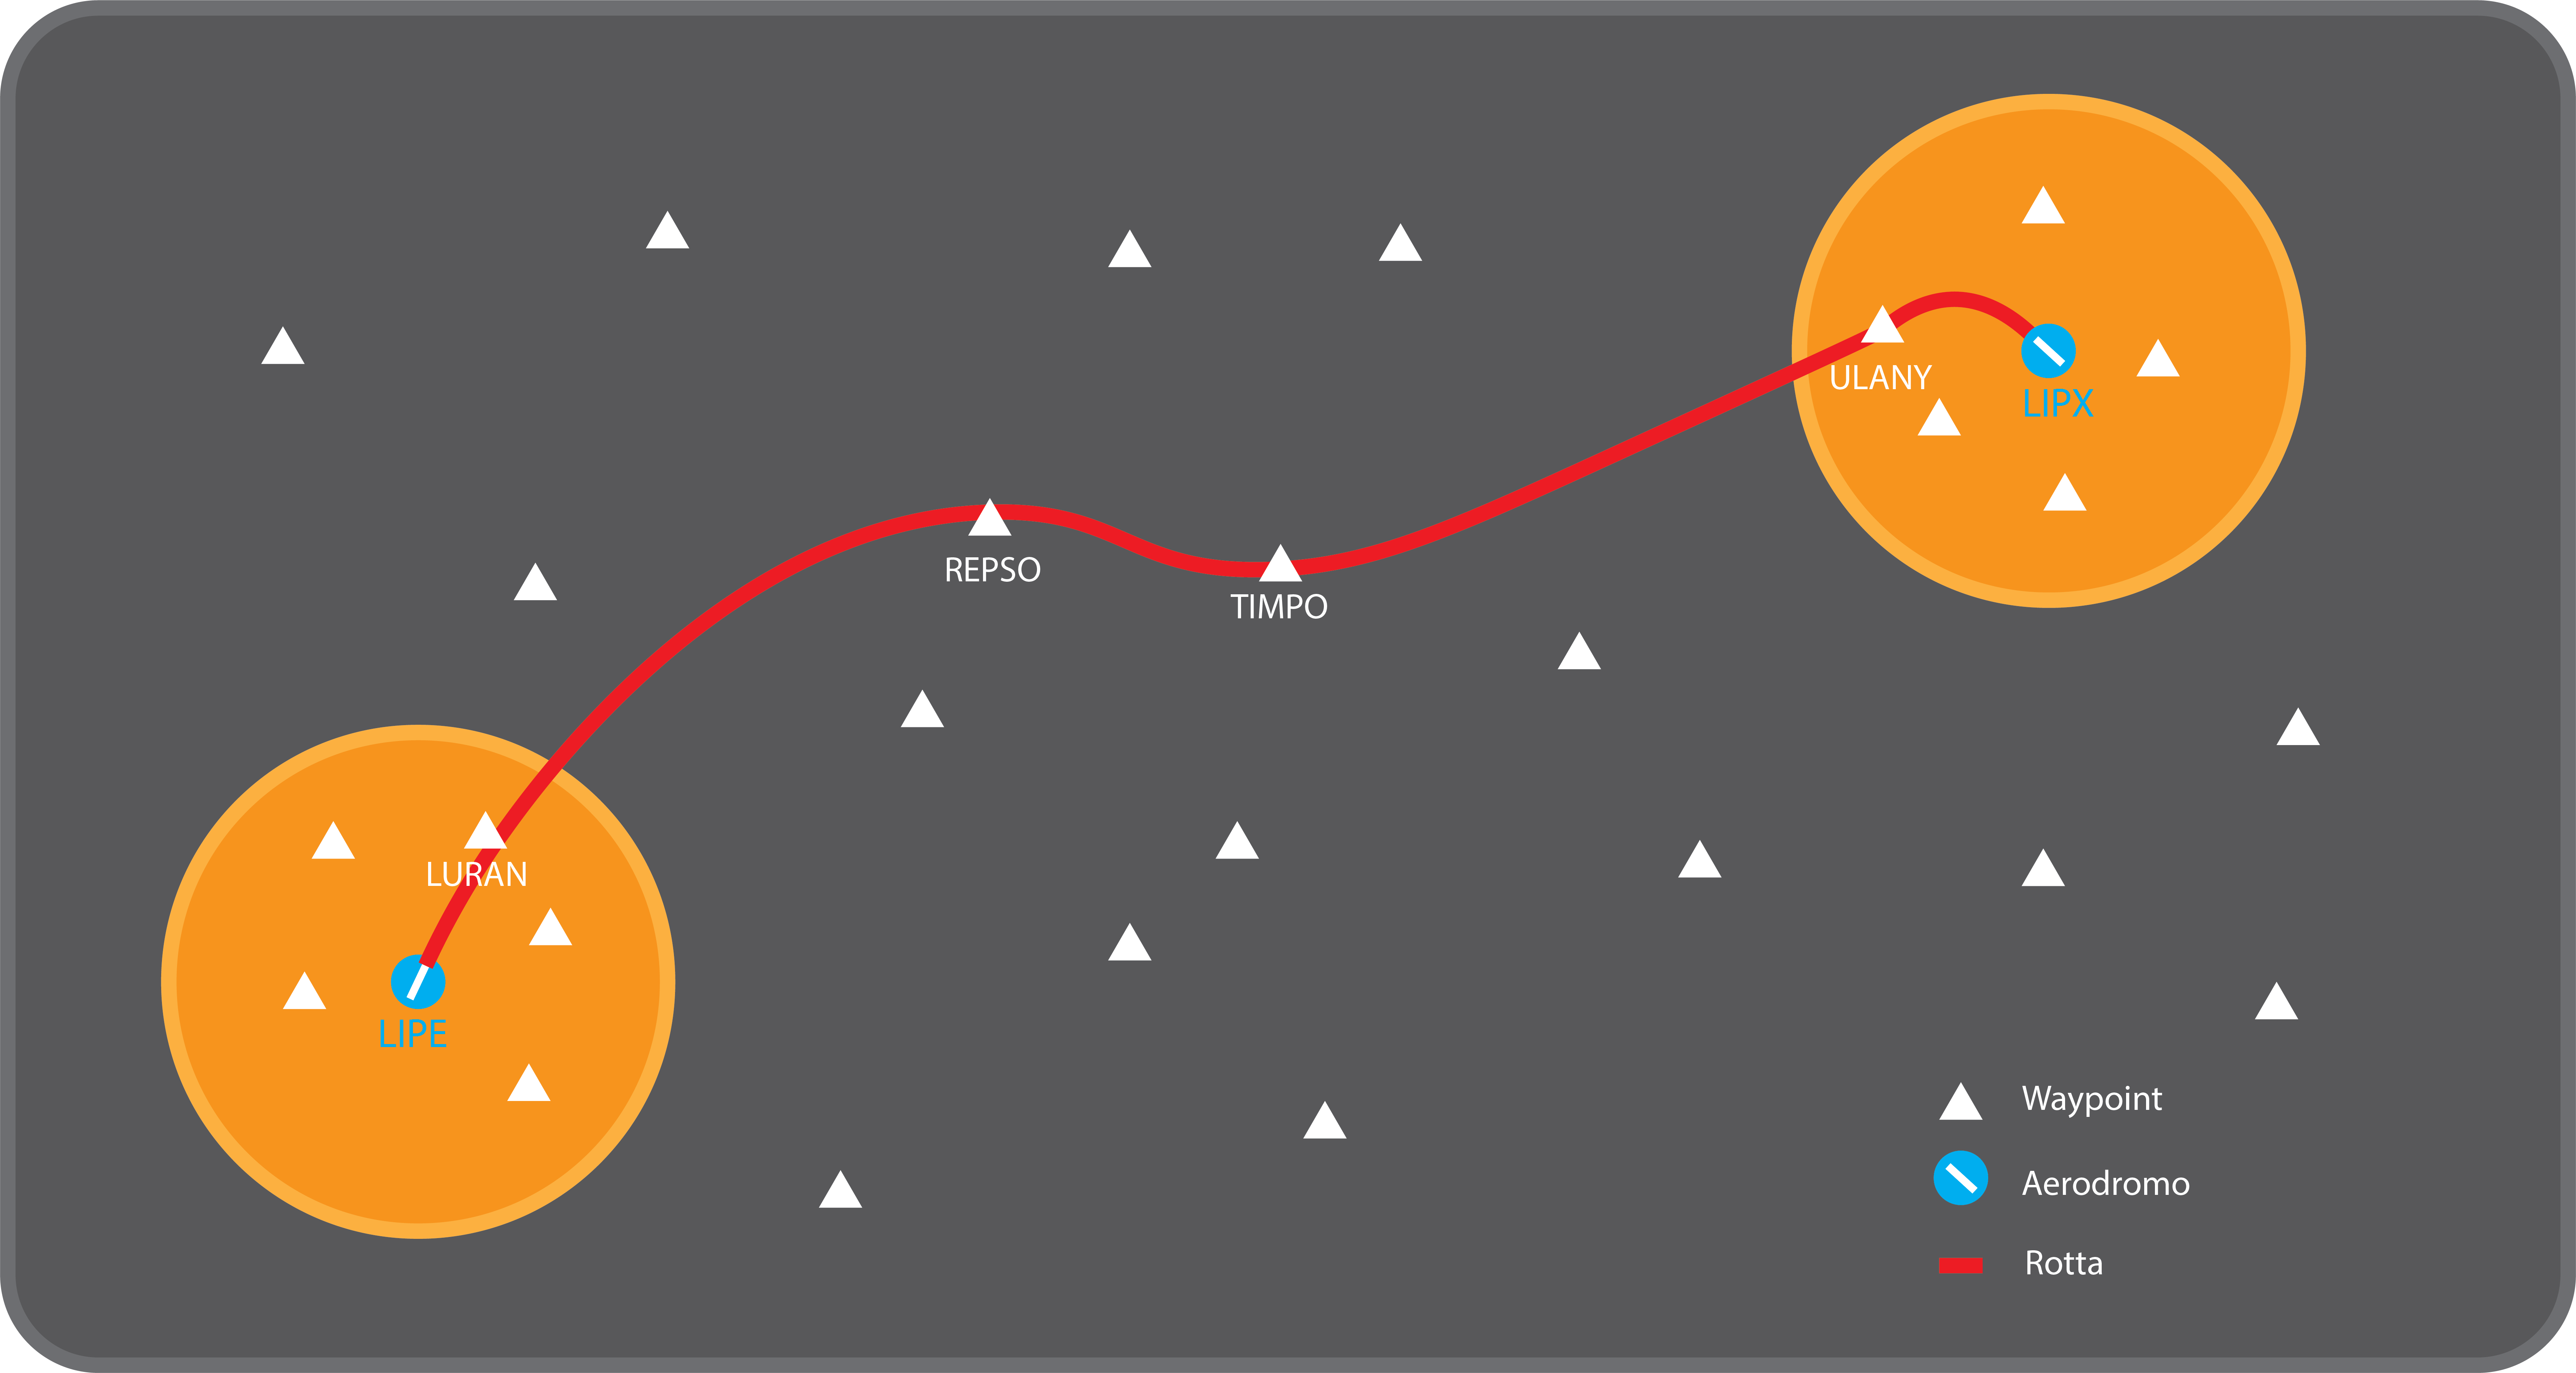
\includegraphics[width=1\textwidth]{figures/esRotta.png}
  \caption{"Un esempio di una rotta e dei settori attraversati"}
  \label{fig:example}
\end{figure}
Ogni controllore è autorizzato a lavorare solamente in posizioni per le quali ha l’abilitazione inoltre gli possono essere allocati turni in posizioni appartenenti al centro in cui lavora.
Esistono due tipi di turni, Il primo, di lavoro mentre il secondo di standby, quest'ultimo è necessario per garantire ridondanza, in caso di imprevisti (e.g. controllore malato, traffico eccessivo)
per ogni 3 turni di lavoro è necessario un lavoratore che copre il turno in standby.
Ogni traffico aereo deve compilare un piano di volo almeno 3 ore prima della partenza, ogni piano di volo contiene il tipo di aeromobile, l'aerodromo di partenza, quello di arrivo e la lista di waypoint che attraverserà.
Ogni punto appartiene ad un settore, i settori possono essere raggruppati o divisi al fine di spartire il carico di lavoro tra più posizioni.
\chapter{Rilevamento delle ambiguità e correzioni proposte}

\chapter{Definizione delle specifiche in linguaggio naturale ed estrazione dei concetti principali}
